
%
%  $Description: Author guidelines and sample document in LaTeX 2.09$
%
%  $Author: Madera $
%  $Date: 2013/06/03 15:20:59 $
%  $Revision: 1.4 $
%

\documentclass[times, 10pt,twocolumn, a4paper]{article}
\usepackage{latex8}
\usepackage{times}
\usepackage{amsmath}
\usepackage{graphicx}
\usepackage[spanish]{babel}

%\documentstyle[times,art10,twocolumn,latex8]{article}

%-------------------------------------------------------------------------
% take the % away on next line to produce the final camera-ready version
\pagestyle{empty}

%-------------------------------------------------------------------------
\begin{document}

\title{\ Algoritmo de estimaci\'on
       de compatibilidad entre parejas humanas}

\author{Quetzali Madera\\
Instituto Tecnol\'ogico de Tijuana\\ Maestr\'ia en ciencias computacionales \\ Tijuana, Baja California Mexico\\ quetz1@msn.com\\}


\maketitle
\thispagestyle{empty}

\begin{abstract}
En ocasiones es dif\'icil conseguir pareja porque se est\'a muy ocupado y puede no haber tiempo para salir con diferentes personas con la intenci\'on de conocerlas. Una persona en promedio puede salir con 7 individuos antes de elegir uno para comenzar una relaci\'on. Este algoritmo predice posibles relaciones duraderas entre 2 personas utilizando una red neuronal Feed-forward con el algoritmo de aprendizaje Levenberg-Marquardt y una serie de datos de parejas con una relaci\'on mayor a 2 a\~nos, de esta forma se reduce el esfuerzo y el tiempo que se invierte en la b\'usqueda de una pareja ideal. 
\end{abstract}



%-------------------------------------------------------------------------
\Section{Introduci\'on}

Una persona puede salir con 7 individuos antes de elegir a uno para comenzar una relaci\'on y esta relaci\'on puede no ser necesariamente una relaci\'on de largo plazo o duradera. El algoritmo que se explicar\'a en este articulo predice posibles relaciones duraderas entre 2 personas utilizando una red neuronal Feed-forward con el algoritmo de aprendizaje Levenberg-Marquardt y una serie de datos de parejas con una relaci\'on mayor a 2 a\~nos, de esta forma se reduce el esfuerzo y el tiempo que se invierte en la b\'usqueda de una pareja ideal.

%-------------------------------------------------------------------------
\SubSection{Red neuronal}

La redes neuronales son un paradigma de aprendizaje y procesamiento autom\'atico inspirado en la forma en que funciona el sistema nervioso de los animales. Se trata de un sistema de interconexi\'on de neuronas que colaboran entre s\'i para producir un est\'imulo de salida. En inteligencia artificial es frecuente referirse a ellas como redes de neuronas o redes neuronales. La estructura de una red neuronal se puede apreciar en la figura \ref{estructura}  \\

Una red neuronal se compone de unidades llamadas neuronas. Cada neurona recibe una serie de entradas a trav\'es de interconexiones y emite una salida. Esta salida viene dada por tres funciones:
    \begin{itemize}
         \item Una funci\'on de propagaci\'on (tambi\'en conocida como funci\'on de excitaci\'on), que por lo general consiste en el sumatorio de cada entrada multiplicada por el peso de su interconexi\'on (valor neto). Si el peso es positivo, la conexi\'on se denomina excitatoria; si es negativo, se denomina inhibitoria.

         \item Una funci\'on de activaci\'on, que modifica a la anterior. Puede no existir, siendo en este caso la salida la misma funci\'on de propagaci\'on.

         \item Una funci\'on de transferencia, que se aplica al valor devuelto por la funci\'on de activaci\'on. Se utiliza para acotar la salida de la neurona y generalmente viene dada por la interpretaci\'on que queramos darle a dichas salidas. Algunas de las m\'as utilizadas son la funci\'on sigmoidea (para obtener valores en el intervalo [0,1]) y la tangente hiperb\'olica (para obtener valores en el intervalo [-1,1]).
    \end{itemize}

Una red neurona es similar al cerebro humano en dos aspectos:
    \begin{itemize}
         \item El conocimiento es adquirido por la red a trav\'es de un proceso de aprendizaje.
         \item Los pesos sin\'apticos o fuerza con que est\'an inter-conectadas las neuronas se utilizan para almacenar la informaci\'on
    \end{itemize}
   
    \begin{figure}[ht!]
	\centering
	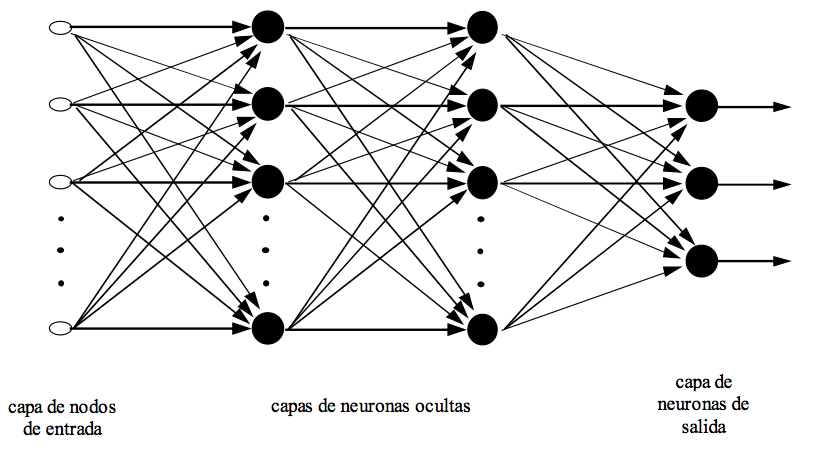
\includegraphics[width=90mm]{rn.png}
	\caption{Estructura de una red neuronal}
	\label{estructura}
    \end{figure}


    
%-------------------------------------------------------------------------
\SubSection{Similitud por Coseno}

Coseno similitud es una medida de similitud entre dos vectores de un espacio de producto interior que mide el coseno del \'angulo entre ellos. El coseno de 0\hspace{-1.5mm}$\phantom{a}^{\circ}$ es 1, y es inferior a 1 para cualquier otro \'angulo. Es por lo tanto un juicio de orientaci\'on y no magnitud: dos vectores con la misma orientaci\'on tienen una similitud coseno de 1, dos vectores a 90\hspace{-1.5mm}$\phantom{a}^{\circ}$ tener una similitud de 0, y dos vectores diametralmente opuestas tienen una similitud de -1, independiente de su magnitud. Coseno similitud se utiliza sobre todo en el espacio positivo, donde el resultado se limita de forma ordenada en \lbrack 0,1\rbrack. \\

Tenga en cuenta que estos l\'imites se aplican para cualquier n\'umero de dimensiones, y coseno similitud se utilizan m\'as com\'unmente en los espacios positivos de alta dimensi\'on. Por ejemplo, en la recuperaci\'on de la informaci\'on, cada t\'ermino se asigna te\'oricamente una dimensi\'on diferente y un documento se caracteriza por un vector, donde el valor de cada dimensi\'on se corresponde con el n\'umero de veces que t\'ermino aparece en el documento. Coseno similitud se da una medida \'util de la similitud de ambos documentos es probable que sean en cuanto a su objeto.\\

La t\'ecnica tambi\'en se utiliza para comparar los documentos en la miner\'ia de texto. Adem\'as, se utiliza para medir la cohesi\'on dentro de las agrupaciones en el \'ambito de la miner\'ia de datos. Una de las razones de la popularidad de coseno similitud es que es muy eficiente para evaluar, sobre todo para los vectores de escaso, ya que s\'olo las dimensiones no-cero necesitan ser consideradas.\\

Dados dos vectores de atributos, A y B, la similitud del coseno, \(cos(\theta)\), se representa mediante un producto de punto y magnitud como:
\\ \\
  
\( similaridad = cos(\theta) = {A\cdot B\over \parallel A \parallel \parallel B \parallel} \) \\

%-------------------------------------------------------------------------
\SubSection{MATLAB}

MATLAB (abreviatura de MATrix LABoratory, "laboratorio de matrices") es una herramienta de software matem\'atico que ofrece un entorno de desarrollo integrado (IDE) con un lenguaje de programaci\'an propio (lenguaje M). Est\'a disponible para las plataformas Unix, Windows y Mac OS X.
Entre sus prestaciones b\'asicas se hallan: la manipulaci\'on de matrices, la representaci\'on de datos y funciones, la implementaci\'on de algoritmos, la creaci\'on de interfaces de usuario (GUI) y la comunicaci\'on con programas en otros lenguajes y con otros dispositivos hardware.\\

El paquete MATLAB dispone de dos herramientas adicionales que expanden sus prestaciones, a saber, Simulink (plataforma de simulaci\'on multidominio) y GUIDE (editor de interfaces de usuario - GUI). Adem\'as, se pueden ampliar las capacidades de MATLAB con las cajas de herramientas (toolboxes); y las de Simulink con los paquetes de bloques (blocksets).
Es un software muy usado en universidades y centros de investigaci\'on y desarrollo. En los \'ultimos a\~nos ha aumentado el n\'umero de prestaciones, como la de programar directamente procesadores digitales de se�al o crear c\'odigo VHDL.

%-------------------------------------------------------------------------

\Section{Objetivo}

Desarrollar un algoritmo capaz de sugerir una persona a un usuario para entablar una relaci\'on de pareja que pueda ser duradera con los datos aportados por la red social Facebook respecto a este usuario. Una pareja duradera se considera posible si es capaz de permanecer m\'as de 2 a\~nos en una relaci\'on afectuosa.

%-------------------------------------------------------------------------

\Section{Aplicaciones}

Este algoritmo puede introducirse en aplicaciones para Facebook para generar posibles relaciones de compatibilidad entre usuarios, estas relaciones pueden ser sentimentales y con algunas modificaciones se puede sugerir otra clase de relaciones como sociedades de negocios o amistades.

%------------------------------------------------------------------------
\Section{Desarrollo}

Los datos de la entrada a la red neuronal son un vector de 6 posiciones que representan los valores de cada uno de los datos del usuario (Nombre, edad, fotos, amigos, post, me gusta, comentarios). Dado que el rango de los n\'umeros que representan los datos es muy grande, los datos se normalizar\'on antes de introducirlos al vector
de la red neuronal. La red neuronal se entrena 20 veces con esos datos utilizando el algoritmo de aprendizaje
Levenberg-Marquardt. La red neuronal tiene 6 neuronas de entrada,  2 capas ocultas: una con 10 neuronas y otra con 6 neuronas y 6 neuronas en la capa de salida, la funci\'on de activaci\'on es tangente sigmoidal en la capa oculta y en la capa de salida una funci\'on lineal.\\

Para comparar el vector de salida con las personas almacenadas y encontrar la similitud entre los datos se utiliz\'o similitud por coseno, una vez obtenida la similitud de los vectores se busca el nombre de la persona a la que corresponda ese vector y de esa forma se puede imprimir en pantalla el nombre de la persona que la red neurona considera ideal para el usuario seg\'un los datos proporcionados. \\

Si se desarrollara una aplicaci\'on para Facebook la salida final se podr\'ia mantener en forma de vector sin utilizar similitud por coseno. y de esa forma presentar las caracter\'isticas de la persona ideal para despu\'es comparar con la base de datos de las amistades de ese usuario. La similitud por coseno nos da la ventaja de no necesitar que los datos de la persona sugerida sean estrictamente iguales a la salida del vector.\\

En la figura \ref{redneuronal} se puede observar la estructura de la red neuronal. y datos de entrenamiento mientras que en la figura \ref{interfaz} se muestra la interfaz que se desarroll\'o para capturar los datos de entrada a la red neurona y presentar el nombre de la persona seleccionada como posible pareja duradera.


\begin{figure}[ht!]
	\centering
	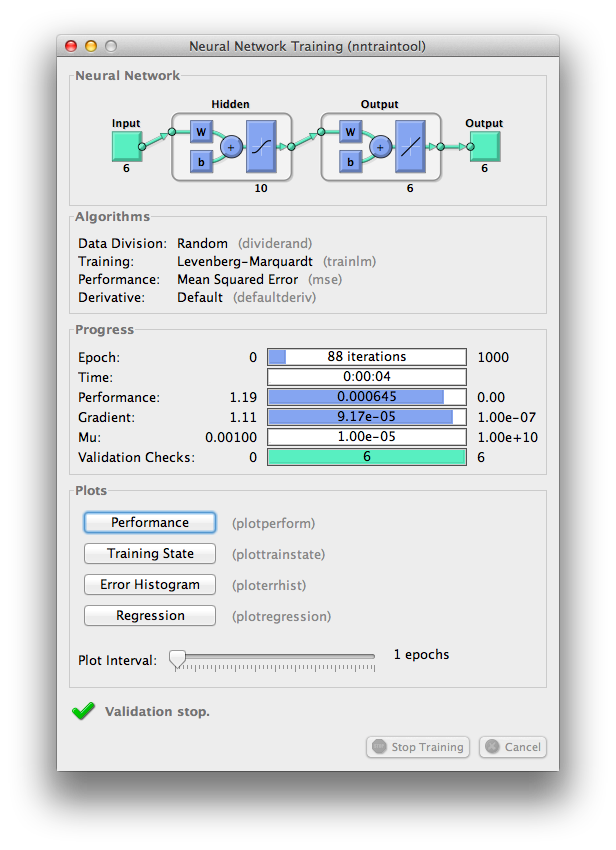
\includegraphics[width=90mm]{entrenamiento.png}
	\caption{Entrenamiento de la red neuronal}
	\label{redneuronal}
    \end{figure}
    
    \begin{figure}[ht!]
	\centering
	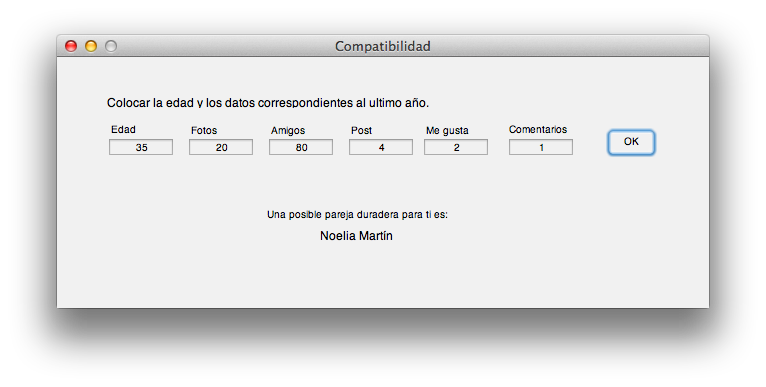
\includegraphics[width=90mm]{interfaz1.png}
	\caption{Interfaz de usuario para ingresar los datos}
	\label{interfaz}
    \end{figure}


%------------------------------------------------------------------------

\SubSection{Datos}

Se proporcionar\'on datos de la red social Facebook de 30 personas: 15 parejas con relaci\'on a largo plazo (m\'as de 2 a\~nos).

Los datos proporcionados son los siguientes:
    \begin{itemize}
         \item Nombre.
         \item Edad.
         \item Fotos.
         \item Amigos.
         \item Cantidad de "Post" (anual).
         \item Cantidad de "Me gusta" (anual).
         \item Comentarios de los post (anual).\\
    \end{itemize}

Los datos se normalizaron para que la entrada a la red neuronal estuviera en un rango de 0 a 1:
Cada dato se dividi\'o entre el dato mas grande de su conjunto. En la figura \ref{datos} se muestran los datos del entrenamiento: de lado izquierdo los datos est\'an sin normalizar y los datos de lado derecho son los datos normalizados.

 \begin{figure}[ht!]
	\centering
	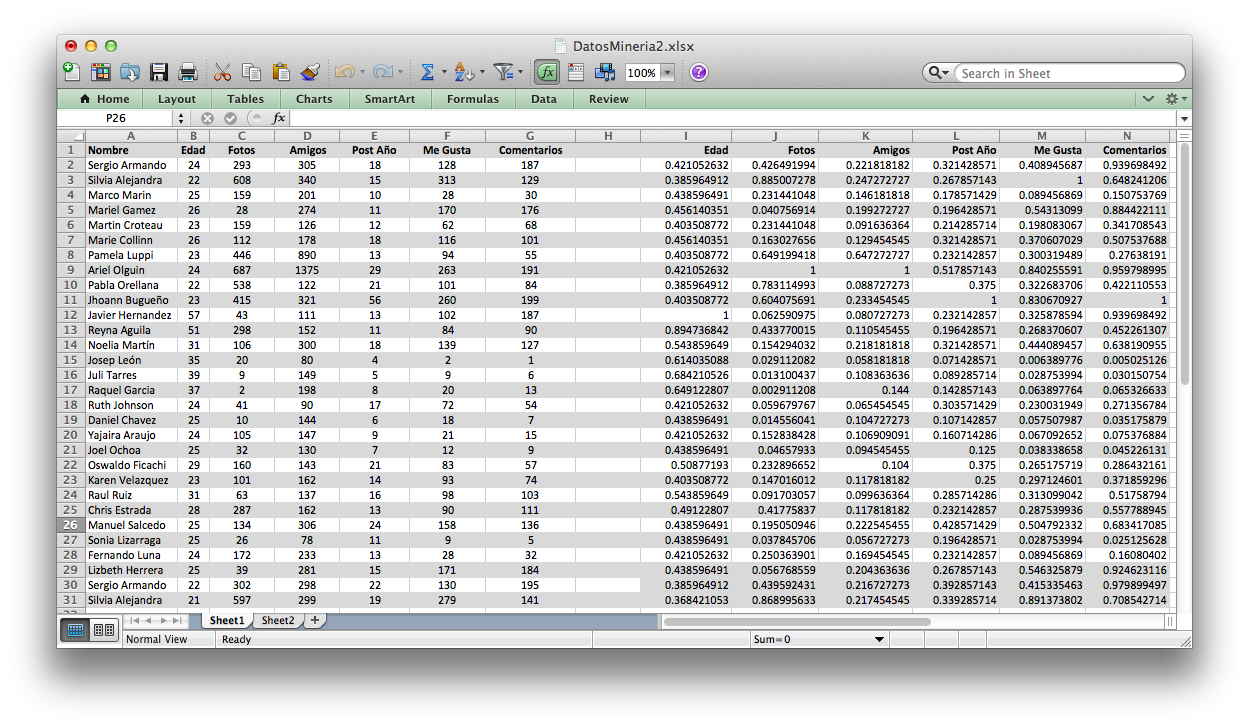
\includegraphics[width=90mm]{datos.png}
	\caption{Tabla de datos}
	\label{datos}
    \end{figure}
    
%-------------------------------------------------------------------------
\Section{Resultados}

Se desarrollo el algoritmo Compatibilidad.m para el entorno MATLAB 2012b. En \'el se ha programado una red neurona con 6 neuronas de entrada y 6 neuronas de salida. Tambi\'en dispone de dos capas ocultas una con 10 neuronas y otra con 6 neuronas. Se a utilizando el algoritmo de aprendizaje Levenberg-Marquardt. En la figura \ref{res} se muestran los resultados de las pruebas con los datos de Facebook.\\

Para probar el algoritmo con datos que no estuvieran en las pruebas, se buscaban los datos de alguna otra pareja de personas con una relaci\'on a largo plazo con la que no se hubiese entrenado antes y estos datos se colocaban en el vector de entrada por medio de la  interfaz gr\'afica, una vez que suger\'ia a una persona como pareja duradera se revisaban los datos de la sugerencia, se comparaban con los datos de la pareja de la persona la cual se introdujo como vector y en todas nuestras pruebas los datos del vector resultante fueron muy similares a los datos de la pareja introducida, por lo que concluimos que los resultados son satisfactorios.

\begin{figure}[ht!]
	\centering
	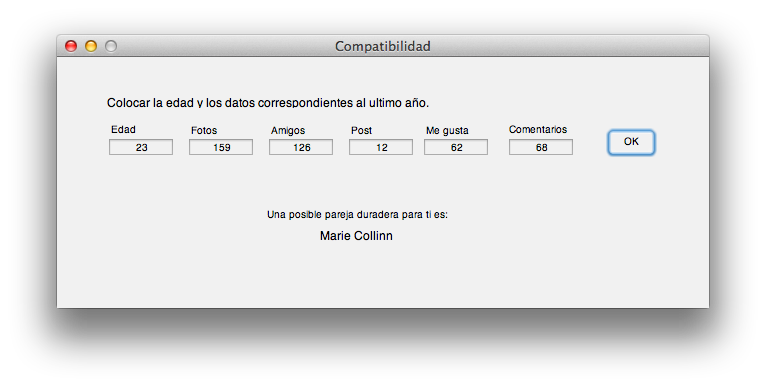
\includegraphics[width=90mm]{res1.png}
	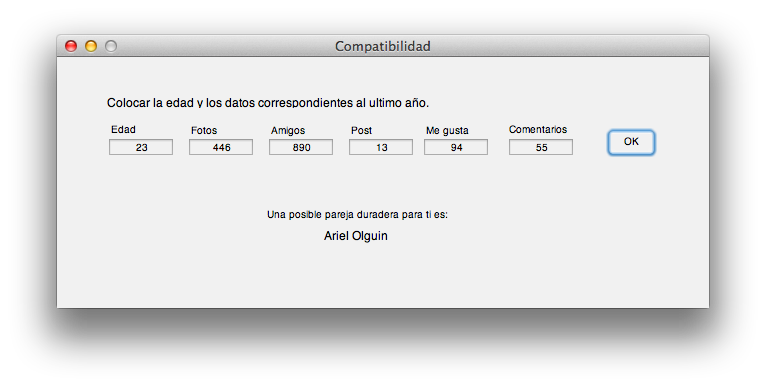
\includegraphics[width=90mm]{res2.png}
	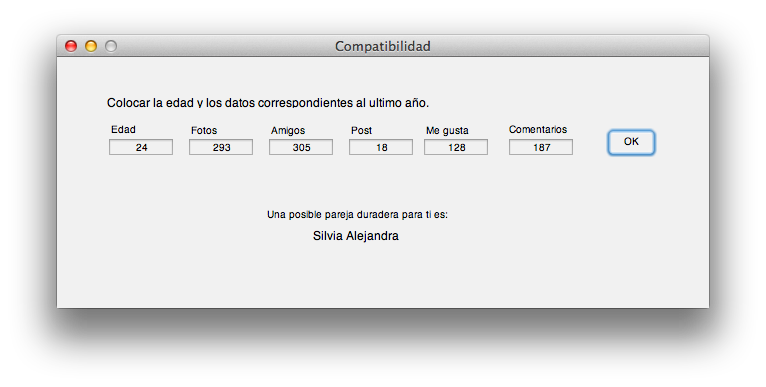
\includegraphics[width=90mm]{res3.png}
	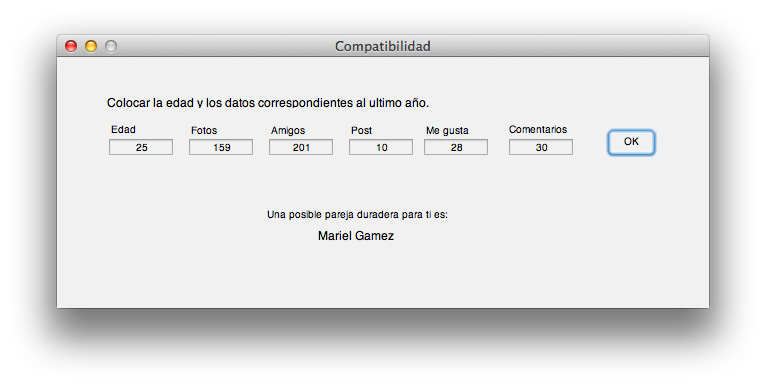
\includegraphics[width=90mm]{res4.png}
	\caption{Resultados de la Compatibilidad}
	\label{res}
    \end{figure}
  %-------------------------------------------------------------------------
  
  \Section{Concluciones}

Los resultados fuer\'on muy satisfactorios y la red neuronal trabaja estupendamente.Las redes neuronales son una excelente opci\'on cuando se trata de problemas de b\'usqueda de caracter\'isticas o patrones entre individuos. En este art\'iculo se desarroll\'o un proyecto relacionado con la redes sociales y la compatibilidad de individuos, pero este mismo m\'etodo se puede utilizar en otra clase de problemas semejantes. \\

El desarr\'ollo fue un poco m\'as complicado de lo que se hab\'ia predicho porque se ignoraban algunos conceptos como las posiciones del vector de entrada, y el manejo de la similaridad entre vectores. Una vez que se hcomprendi\'o, el desarrollo fue m\'as fluido. \\

En general el desarrollo del proyecto fue interesante y provechoso dado que se comprendieron muchos detalles previamente estudiados. En general los resultados fueron muy satisfactorios pero aun hay que hacer algunas modificaciones para optimizar el algoritmo y utilizaci\'on como una aplicaci\'on.

%-------------------------------------------------------------------------

\Section{Referencias}

    \begin{itemize}
         \item Singhal, Amit (2001). Modern Information Retrieval: A Brief Overview. Bulletin of the IEEE Computer Society Technical Committee on Data Engineering.
         \item P.-N. Tan, M. Steinbach and V. Kumar, Introduction to Data Mining , Addison-Wesley (2005), ISBN.
         \item Perceptr�n multicapa, Redes de Neuronas Artificiales, UC3M, RAI 2012.
         \item Haykin, Simon (1998). Neural Networks: A Comprehensive Foundation (2 edici�n). Prentice Hall. ISBN 0132733501
         \item Emiliano Aldabas-Rubira; �Introducci�n al reconocimiento de patrones mediante re- des neuronales�. JCEE, 2002.
    \end{itemize}

%-------------------------------------------------------------------------
\Section{Agradecimientos}

En esta secci\'on quiero agradecer a mi maestro el Dr. Mario Garcia Valdez por todo el conocimiento que me ha dado, a mi novio Amaury Hern\'andez \'Aguila por su aportaci\'on explic\'andome la similitud por coseno y porque es el mejor novio del mundo, y a mis padres porque me brindan techo y comida para que yo avance con mis estudios de maestr�a.\\

Un agradecimiento especial a CONACYT porque me ha otorgado una beca y no hay mejor motivaci\'on que eso para hacer investigaciones.
%-------------------------------------------------------------------------

\nocite{ex1,ex2}
\bibliographystyle{latex8}
\bibliography{latex8}

\end{document}
